\chapter{Discussion and Further Work}

This thesis presents promising results for a potential application of differentiable ray
tracing~\cite{li2018differentiable} in deep learning models. Our results in
Chapter~\ref{ch:experiment} demonstrate the extent of our model's generative ability while also
outlining the limitations of our technique. In this section, we discuss the source of these
limitations and suggest potential improvements to be explored as further work.

\section{Distortion in mesh parameterization} \label{sec:distortion}

In Section \ref{sec:uv-embedding}, we justified a simple UV-embedding which utilized the
spherical parameterization of the points on the surface while noting the poor distortion
qualities of the embedding. For the scope of this thesis, we focused on improving the
learning task, and were not able to address the distortion artifacts appropriately. As
future work, it is more desirable to use a better UV-embedding parameterization that
minimizes surface distortion, such as Sander et al.'s solution of running an optimization
to minimize the stretch metric of the embedding~\cite{sander2001texture},

\section{Generalizing the model for real images}

Although the ultimate goal of our model is to learn texture-maps of surface weathering based
on exemplar images of real cars, we found directly training GANs on a dataset of real
images to be difficult due to volatility of the model to \emph{mode collapse}. There are many
details of real scenes have which are very difficult to emulate in a 3D scene and vice versa.

An example of a fundamental difference between ray traced images and real scene images is
Monte-Carlo noise artifacts produced in ray traced images. Monte-Carlo noise is caused by the
stochastic nature of Monte-Carlo sampling and leads to noisy images as shown in Figure
\ref{fig:monte-carlo}. Although this noise decreases with higher MC sampling rates, the SNR improves
roughly with $O(n^{1/2})$ where $n$ is the sampling rate. Therefore, computationally, it
becomes infeasible to keep increasing the samples we use per pixel. However, unless the
dataset has noticeably less Monte-Carlo noise compared to the input dataset, the discriminator
learns to distinguish the fake and real images using the noise profile of its input image in a
similar fashion as we showed in Chapter~\ref{ch:experiment}.

\begin{figure}
    \centering
    \caption{Monte-Carlo sub-sampling per pixel has a huge effect on the resultant render.
        Training the model using a low Monte-Carlo sub-sampling rate causes the discriminator
        to \emph{mode collapse} due to the discrepancy in render quality.}
    \label{fig:monte-carlo}
    \vspace{0.2in}
    \begin{subfigure}[t]{0.32\linewidth}
        \centering
        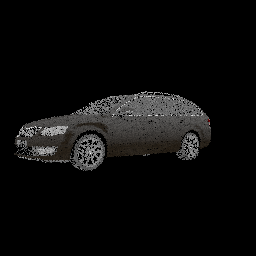
\includegraphics[width=\linewidth]{graphics/mc1.png}
        \caption{1 sub-sample}
    \end{subfigure}
    \begin{subfigure}[t]{0.32\linewidth}
        \centering
        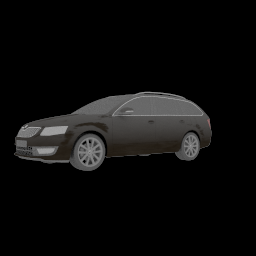
\includegraphics[width=\linewidth]{graphics/mc200.png}
        \caption{200 sub-samples}
    \end{subfigure}
\end{figure}

This artifact is only one of many difficulties associated with the problem of extending our
model to train on real images. However, our current hypothesis is that the discriminator uses
the most easily learnable feature to distinguish between real and fake images. If we keep
eliminating the most easily learnable feature that is not the dirt texture on the surface of the
car, we hope that the discriminator will eventually be forced to learn to distinguish clean
cars from dirty ones.

\section{Differentiable ray tracing in deep learning applications}

This thesis primarily focused on generating simple diffuse textures. But our general method
applies to learning arbitrary scene description parameters using deep learning models.
Improving the surface shader complexity of our model, such as adding learnable specular
components and normal maps, would add more expressiveness to the output textures. Furthermore,
we can also attempt to train a model which learns shapes of surfaces in 3D using images of
these shapes. Regardless of the specific application in mind, we hope that our work can be a
good baseline for deep learning models featuring differentiable ray tracing in future research.
